\section{Complementary-filtered residual world model}

\begin{figure*}[t]
\centering
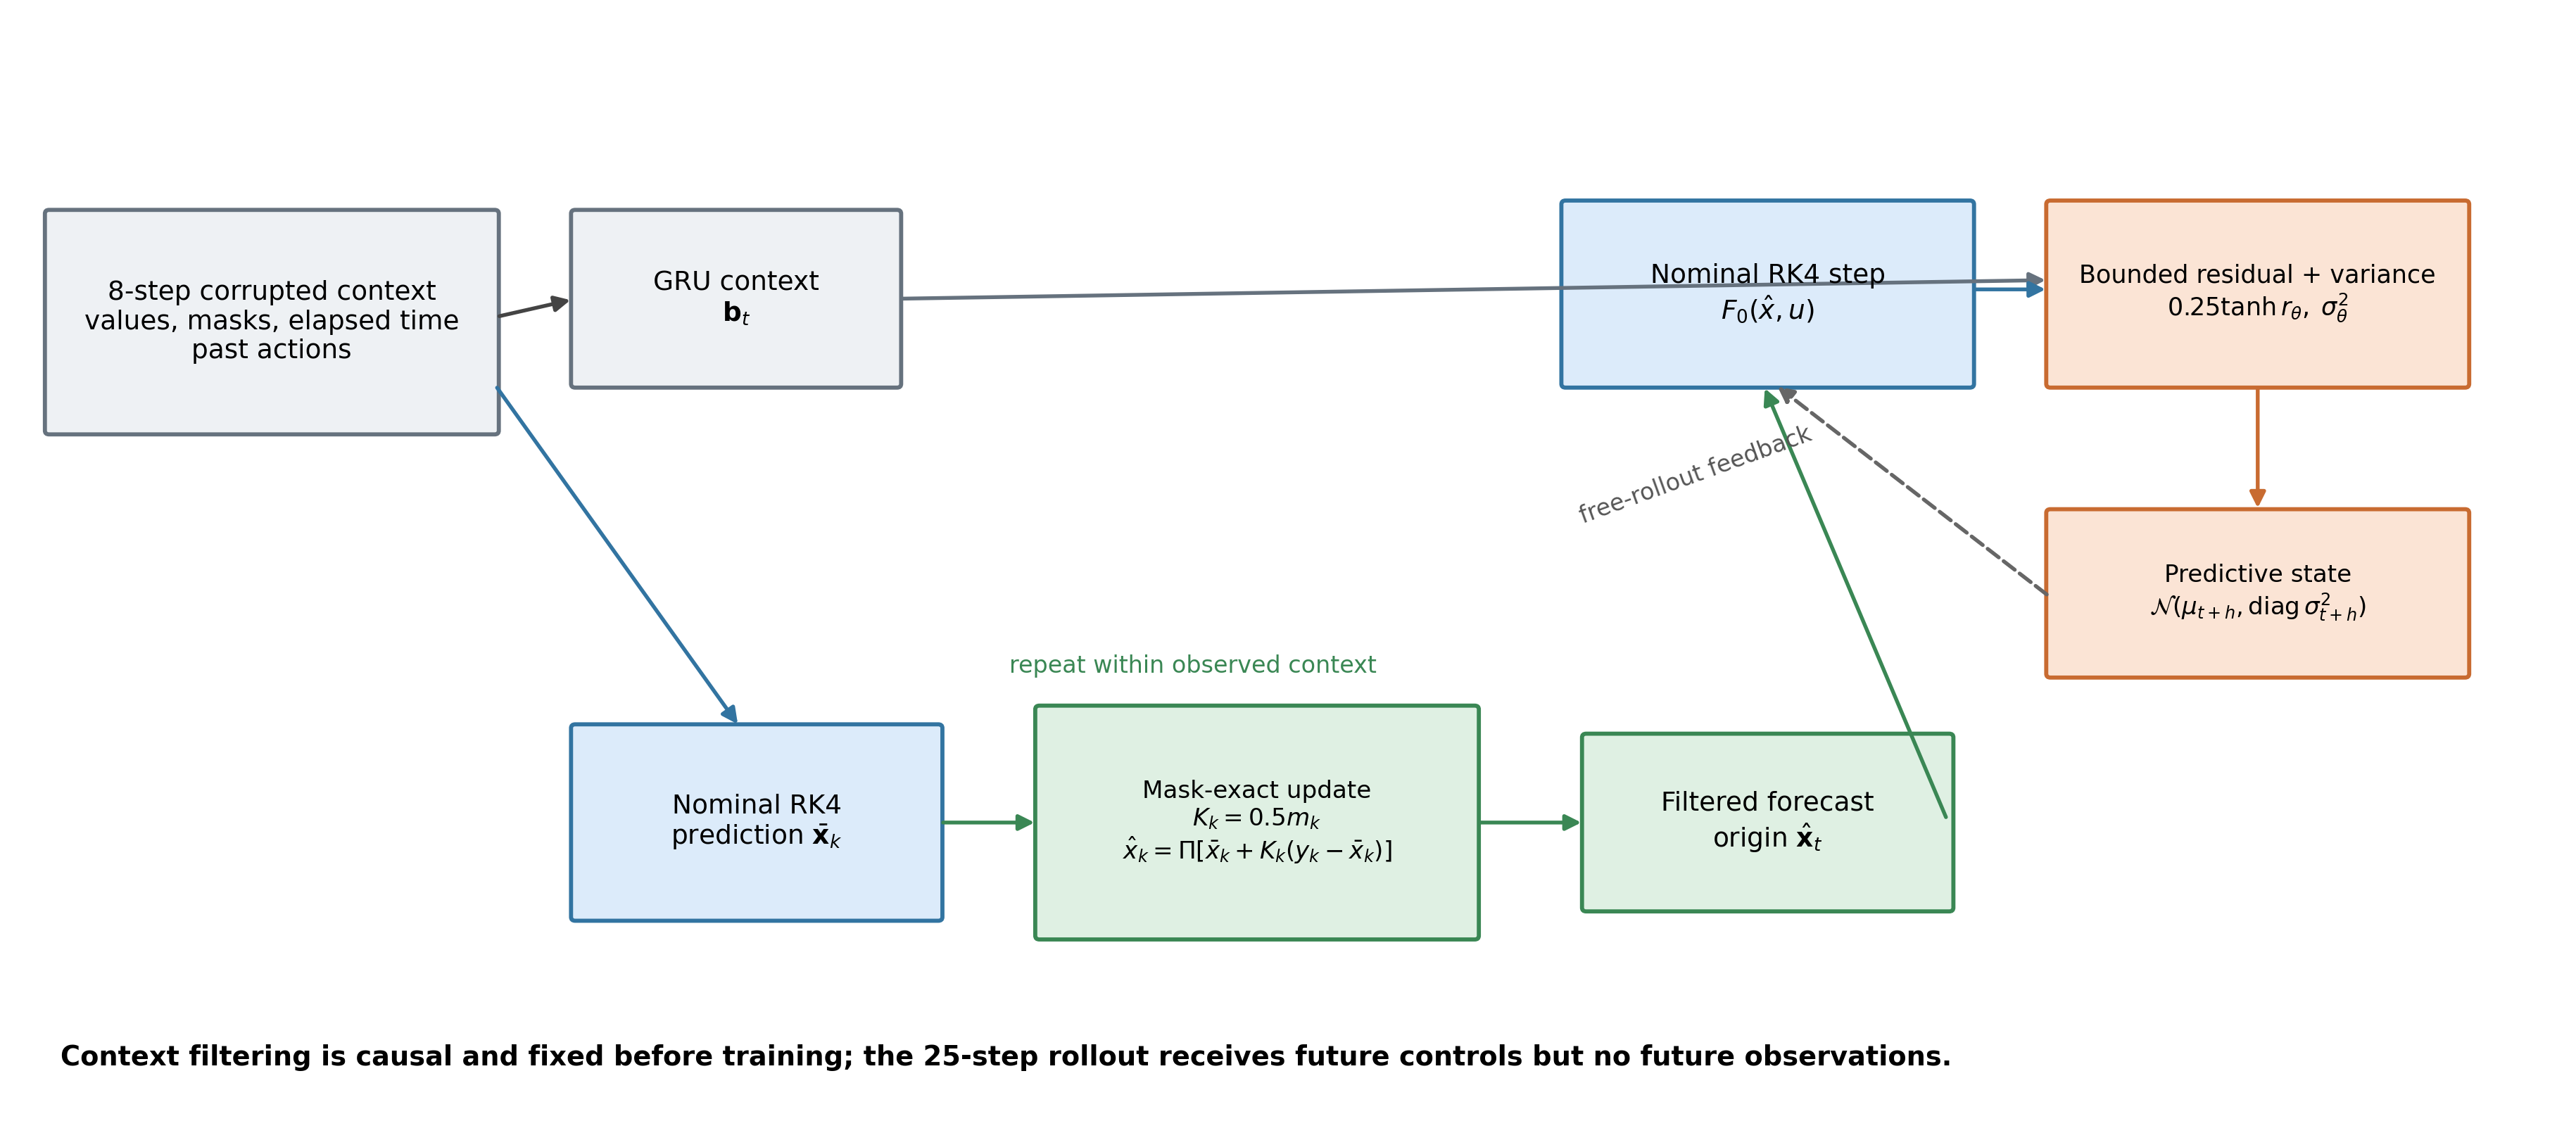
\includegraphics[width=0.96\textwidth]{figures/figure1_method.png}
\caption{Causal data flow of \method{}. A fixed complementary update is applied only inside the observed context. Missing channels receive exactly zero measurement gain. The filtered forecast origin then initializes a probabilistic nominal-physics plus neural-residual transition, which is rolled out freely for 25 steps using known future controls and no future observations.}
\label{fig:method}
\end{figure*}

\subsection{Forecasting problem}

Let $\vect{x}_t\in\mathbb{R}^{d_x}$ be a physical state and
$\vect{u}_t\in\mathbb{R}^{d_u}$ a recorded control. The observation available
to the model is
\begin{equation}
 \vect{y}_t=\vect{m}_t\odot(\vect{x}_t+\boldsymbol{\epsilon}_t),
\end{equation}
where $\vect{m}_t\in\{0,1\}^{d_x}$ is a channel-wise availability mask and
$\boldsymbol{\epsilon}_t$ is observation noise. Missing entries are filled
causally by the latest available value, producing $\tilde{\vect{y}}_t$; the
mask and elapsed time since observation $\boldsymbol{\delta}_t$ remain explicit
inputs, so an imputed value is never represented as a fresh measurement.

At forecast origin $t$, the model receives eight context states and their past
controls,
\begin{equation}
 \mathcal C_t=\{\tilde{\vect y}_{t-7:t},\vect m_{t-7:t},
 \boldsymbol\delta_{t-7:t},\vect u_{t-7:t-1}\},
\end{equation}
together with known future controls $\vect u_{t:t+H-1}$. It estimates a
diagonal predictive distribution for $\vect{x}_{t+1:t+H}$ under free rollout,
with $H=25$. Future states or observations are never fed back. All learned
operations use affine statistics estimated from the training split; the
nominal equations are evaluated in physical coordinates and then returned to
normalized coordinates.

\subsection{Mask-exact complementary context filter}

Let $F_0$ be one fourth-order Runge--Kutta step of a nominal controlled
differential equation. Starting from the first imputed context vector, the
filter alternates nominal prediction and measurement update. For context index
$k>t-7$,
\begin{align}
 \bar{\vect x}_{k} &= F_0(\hat{\vect x}_{k-1},\vect u_{k-1}),\\
 \vect K_k &= \alpha\vect m_k,\qquad \alpha=0.5,\\
 \hat{\vect x}_k &= \Pi\!\left[
 \bar{\vect x}_k+\vect K_k\odot
 (\tilde{\vect y}_k-\bar{\vect x}_k)\right].
 \label{eq:complementary-update}
\end{align}
Thus, before projection, an observed channel receives equal weight from the
nominal prediction and the current measurement, while a missing channel has
exactly zero measurement correction. The projection $\Pi$ is the identity
except for the sine--cosine pendulum representation, which is returned to the
unit circle after each update. That joint projection can alter either pendulum
channel even when its own measurement gain is zero, so the implementation does
not claim channel-wise equality to nominal propagation after projection. The
gain is fixed before training and has no access to validation or test outcomes.

In parallel, a GRU encodes
$[\tilde{\vect y}_k,\vect m_k,\log(1+\boldsymbol\delta_k),\vect u_{k-1}]$.
Its last hidden state supplies trajectory context to the forecast transition;
it does not alter the fixed measurement gain. The implementation retains the
same unused gain-head parameterization in every fixed-gain sensitivity model,
so comparisons at gains 0, 0.25, 0.5, 0.75, and 1 do not change nominal
capacity. We do not claim that complementary or Kalman-style filtering is new;
KalmanNet and modern data-assimilation work establish the broader prior art
\cite{revach2022_kalmannet,cheng2023_machine_learning_with_data_assimilation}.
The tested contribution is the use of a prespecified, mask-exact context update
as the forecast origin of a physics-residual probabilistic world model.

\subsection{Probabilistic physics-residual rollout}

The last filtered context state initializes a free rollout. At step $h$,
\begin{align}
 \boldsymbol\mu^{p}_{t+h} &= F_0(\hat{\vect x}_{t+h-1},\vect u_{t+h-1}),\\
 [\vect r_{t+h},\vect \ell_{t+h}] &=
 R_\theta([\hat{\vect x}_{t+h-1},\vect u_{t+h-1},\vect b_{t+h-1}]),\\
 \boldsymbol\mu_{t+h} &= \Pi\!\left[
 \boldsymbol\mu^{p}_{t+h}+0.25\tanh(\vect r_{t+h})\right],\\
 \boldsymbol\sigma^2_{t+h} &=
 \max\!\left\{\exp\!\left(\operatorname{clip}(\vect\ell_{t+h},-8,4)\right),
 10^{-6}\right\}.
 \label{eq:residual-rollout}
\end{align}
The fixed residual scale bounds a single normalized correction but does not
guarantee a bounded trajectory because errors can accumulate. The predicted
mean becomes the next state, and a GRUCell updates $\vect b$ from that mean and
the known control. No sampled state or future target enters the recurrence.

The training loss is the mean diagonal Gaussian negative log likelihood over
all $H$ steps and state channels,
\begin{equation}
 \mathcal L_{\mathrm{NLL}}=
 \frac{1}{2Hd_x}\sum_{h=1}^{H}\sum_{q=1}^{d_x}
 \left[\log(2\pi\sigma^2_{hq})+
 \frac{(x_{hq}-\mu_{hq})^2}{\sigma^2_{hq}}\right].
 \label{eq:nll}
\end{equation}
The one-step ablation applies the same loss only at $h=1$ but is still
evaluated by a 25-step free rollout.

\subsection{Causal execution and computational cost}

For each window, execution follows four deterministic stages. First, the GRU
encodes the imputed context together with masks, elapsed times, and past
controls. Second, Equation~\eqref{eq:complementary-update} advances the nominal
state through the same context and applies the mask-exact correction after each
available observation. Third, the final hidden state and filtered state jointly
initialize the residual recurrence. Fourth, Equation~\eqref{eq:residual-rollout}
is iterated for every known future control; predicted means, rather than samples
or targets, feed the next step. Training backpropagates the multi-step NLL
through this entire causal graph. Evaluation uses the identical graph with
gradients disabled, so teacher forcing is absent from both validation and test
rollouts.

Let $T_c$ denote context length, $H$ forecast horizon, $d_b$ recurrent width,
and $C_{F_0}$ the cost of one nominal RK4 step. Dense recurrent operations cost
$O((T_c+H)d_b^2)$ per trajectory, while nominal propagation costs
$O((T_c+H)C_{F_0})$. Diagonal mean and variance storage is $O(Hd_x)$; recurrent
working memory at inference is $O(d_b+d_x)$. Thus inference grows linearly in
context and horizon. The analysis does not claim asymptotic superiority over
the comparators: the fixed filter adds nominal context steps, and measured
latency is reported as an implementation property rather than a theoretical
speed advantage.

\subsection{Error decomposition and claim boundary}

For an observed scalar channel on which $\Pi$ is the identity, write the
nominal pre-update error as $e_p=\bar x-x$ and measurement error as
$\epsilon=y-x$. Before any non-identity projection, Equation
\eqref{eq:complementary-update} gives the exact post-update error
\begin{equation}
 e_f=(1-\alpha)e_p+\alpha\epsilon.
\end{equation}
If these errors are zero-mean and uncorrelated, then
\begin{equation}
 \mathbb E[e_f^2]=(1-\alpha)^2\mathbb E[e_p^2]
 +\alpha^2\mathbb E[\epsilon^2].
 \label{eq:filter-mse}
\end{equation}
Equal trust is therefore not universally optimal: it helps only when the two
error sources are sufficiently balanced, and a missing channel receives no
direct measurement-error term because its gain is zero. For the pendulum's
joint sine--cosine projection, an additional coupled projection error must be
accounted for, so Equation~\eqref{eq:filter-mse} is not asserted channel-wise
after projection. This conditional identity, rather than an optimal-filter
claim, motivates the fixed-gain sensitivity analysis.

If the rollout transition is locally $L$-Lipschitz and incurs local error
$\eta_h$, the standard recursion yields
\begin{equation}
 \|\hat{\vect x}_{t+H}-\vect x_{t+H}\|
 \le L^H\|\hat{\vect x}_t-\vect x_t\|
 +\sum_{h=0}^{H-1}L^{H-1-h}\eta_h.
\end{equation}
The context filter can reduce only the initial-error term; the residual model
must control subsequent local errors. Neither relation provides an
unconditional stability guarantee or supports claims about visual
representation learning, policy quality, or real-robot transfer.
